\subsection{推理循环与软件栈}

LeRobot 的在线推理是一个持续运行的帧循环：
每一帧依次经历\textbf{观测采集}（\texttt{get\_observation()}）、
\textbf{策略推理}（\texttt{select\_action()}）、
\textbf{指令下发}（\texttt{send\_action()}）和\textbf{等待}四个阶段，
周而复始直到 episode 结束（图~\ref{fig:record-loop}）。
该循环在单个 Python 进程内串行执行，不依赖外部消息中间件，
若以 30\,fps 作为控制目标，则单帧可用时间约为 33.3\,ms。

\begin{figure}[htbp]
  \centering
  \begin{tikzpicture}[>=Stealth,
    stage/.style={
      rectangle, rounded corners=3pt, draw=blue!60, fill=blue!8,
      minimum width=2.8cm, minimum height=1cm, align=center,
      font=\small\bfseries
    },
    sub/.style={
      rectangle, rounded corners=2pt, draw=gray!70, fill=gray!6,
      minimum width=2.6cm, minimum height=0.7cm, align=center,
      font=\footnotesize
    },
    note/.style={font=\scriptsize\itshape, text=gray!80}
  ]
    \node[stage] (obs)  {观测采集\\[-1pt]{\footnotesize\texttt{get\_observation()}}};
    \node[stage, right=1.2cm of obs]  (inf)  {策略推理\\[-1pt]{\footnotesize\texttt{select\_action()}}};
    \node[stage, right=1.2cm of inf]  (act)  {指令下发\\[-1pt]{\footnotesize\texttt{send\_action()}}};
    \node[stage, right=1.2cm of act]  (wait) {等待\\[-1pt]{\footnotesize\texttt{fps\_sleeper()}}};

    \draw[->, thick, blue!60] (obs)  -- (inf);
    \draw[->, thick, blue!60] (inf)  -- (act);
    \draw[->, thick, blue!60] (act)  -- (wait);
    \draw[->, thick, red!60] (wait.north) -- ++(0,0.8) -| (obs.north)
      node[pos=0.25, above, note] {下一帧};

    \node[sub, below=0.65cm of obs] (async)
      {异步读摄像头线程\\[-1pt]{\footnotesize\texttt{async\_read}}};

    \draw[->, thin, gray, dashed] (obs.south) -- (async.north);

    \node[note, right=0.15cm of async.east] {读取最新帧};
    \node[note, below=0.3cm of inf.south] {ACT / PyTorch};
    \node[note, below=0.3cm of act.south] {\texttt{sync\_write} $\to$ 舵机};
  \end{tikzpicture}
  \caption{LeRobot 单帧推理循环流程：观测$\to$推理$\to$执行$\to$等待，周而复始}
  \label{fig:record-loop}
\end{figure}

每个阶段调用不同的软件栈路径（图~\ref{fig:lerobot-stack}）：
\textbf{观测阶段}同时采集摄像头图像和关节角度——
摄像头图像通过 OpenCV 后台线程异步预取，主线程调用 \texttt{async\_read()} 取回已解码帧，
底层经由 V4L2 驱动和内核 \texttt{pselect6} 等待帧就绪；
关节角度由 scservo\_sdk 通过 pyserial 以 \texttt{sync\_read} 指令向舵机总线发起同步读取，
底层经由串口驱动和内核 \texttt{read}/\texttt{write} 系统调用完成半双工通信。
\textbf{推理阶段}将观测张量送入 ACT 策略网络，
由 PyTorch（C10 线程池 + ARM NEON 算子）在 CPU 上完成前向计算，
经由 glibc 和 Linux 内核的 futex 机制协调线程同步。
\textbf{执行阶段}将预测动作通过 scservo\_sdk 以 \texttt{sync\_write} 写回舵机，
路径与观测阶段的关节读取对称。\textbf{等待阶段}由 \texttt{fps\_sleeper} 调用 \texttt{time.sleep()} 补足帧间隔，
底层触发 \texttt{nanosleep} 系统调用使进程主动让出 CPU。

\begin{figure}[H]
  \centering
  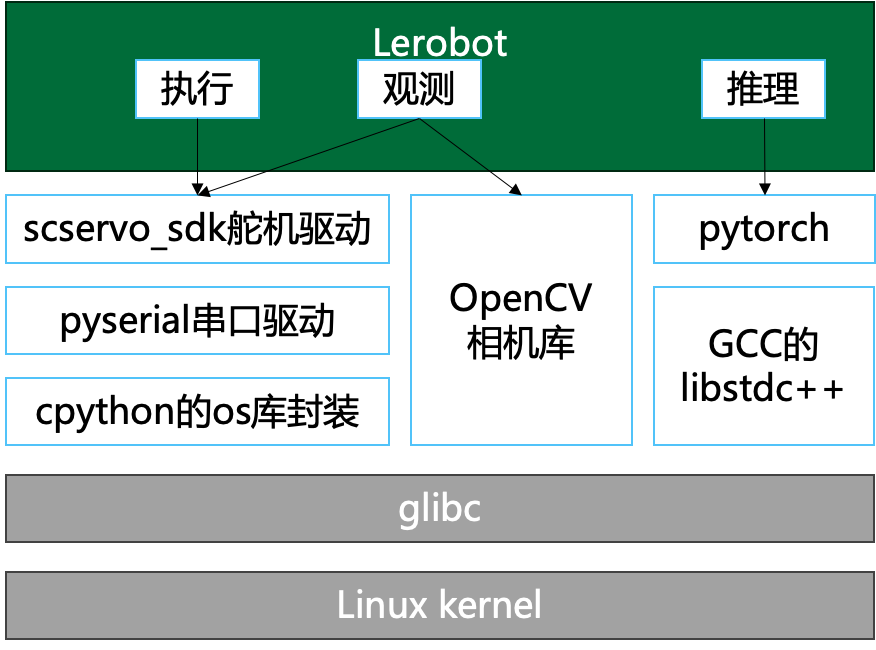
\includegraphics[width=0.9\textwidth]{2_实验环境构建/image/lerobot_stack.png}
  \caption{LeRobot 软件栈四层架构：应用逻辑层$\to$库与驱动层$\to$glibc$\to$Linux 内核}
  \label{fig:lerobot-stack}
\end{figure}

\src{LeRobot软件栈全链路分析.md}
